% titulo: Capítulo III – Metodología de desarrollo
% estado: borrador
% actualizado: 2026-10-19
% Sincronizado con specs/00-producto.md v1.0 el 19-oct-2026 (ver Tesis-Doc/README.md, registro S-nn).

\chapter{Metodología de Desarrollo}\label{cap:metodologia}

% **Regla de este capítulo.** Lo que ya está definido en `specs/` no se copia aquí: se resume y se enlaza. Si un dato de
% este capítulo contradice a `specs/00-producto.md`, prevalece la spec. Las cifras de avance viven en `AVANCE.md`
% y se congelan en este capítulo solo al cierre (Sprint 6).

\section{Tipo y enfoque de la investigación}

Esta tesis es una investigación aplicada con enfoque tecnológico. Eso quiere decir que el resultado no es una teoría sino un programa que se construye y se prueba con una revista real.

\begin{itemize}
  \item El producto es un agente de sugerencias estilísticas que se conecta con OJS y se prueba con la revista Innosoft.
  \item El desarrollo es iterativo e incremental porque en cada sprint se entrega una parte que ya funciona de principio a fin y esa parte se muestra a los editores y se corrige antes de pasar a la siguiente.
  \item La evaluación se hace al final con manuscritos de prueba y con la opinión de los editores sobre las sugerencias que recibieron.
\end{itemize}

\section{Marco de trabajo}

Para organizar el trabajo se combinan tres prácticas que cubren cosas distintas. Scrum ordena el tiempo RICE ordena las prioridades y Spec-Driven Development ordena cómo se escribe cada funcionalidad antes de programarla.

\begin{longtable}{@{}>{\raggedright\arraybackslash}p{0.179\textwidth}>{\raggedright\arraybackslash}p{0.505\textwidth}>{\raggedright\arraybackslash}p{0.237\textwidth}@{}}
\toprule
\textbf{Práctica} & \textbf{Para qué se usa} & \textbf{Artefacto} \\
\midrule
\endfirsthead
\toprule
\textbf{Práctica} & \textbf{Para qué se usa} & \textbf{Artefacto} \\
\midrule
\endhead
\bottomrule
\endfoot
\endlastfoot
\textbf{Scrum} & El trabajo se divide en sprints de dos semanas entre el 14 de septiembre y el 4 de diciembre de 2026 y los dos tesistas hacen a la vez de desarrolladores de Product Owner y de Scrum Master. & Sprint Backlog, Sprint Review, retrospectiva \\
\textbf{RICE} & Cada historia recibe un puntaje que sale de multiplicar alcance impacto y confianza y dividir entre esfuerzo y con ese puntaje se decide qué se hace primero y qué historias forman el \emph{walking skeleton} que es el flujo mínimo de principio a fin. & \texttt{priorizacion\_\allowbreak{}rice\_\allowbreak{}sprint1.\allowbreak{}xlsx} \\
\textbf{Spec-Driven Development (SDD)} & Exige que cada historia tenga una especificación aprobada antes de escribir código; las pruebas se derivan de sus criterios de aceptación. & \texttt{specs/\allowbreak{}US-nn.\allowbreak{}md} \\
\end{longtable}

Cada historia de usuario pasa por el mismo ciclo de seis pasos que son especificar revisar planificar implementar verificar y cerrar. La especificación de una historia es un documento corto que se escribe antes del código y que va cambiando de estado conforme avanza.

\begin{itemize}
  \item Empieza en borrador cuando uno de los tesistas la escribe.
  \item Pasa a en revisión cuando el otro tesista la lee y deja comentarios.
  \item Pasa a aprobada cuando los dos están de acuerdo y recién ahí se puede programar.
  \item Pasa a implementada cuando el código y sus pruebas están en la rama principal.
  \item Pasa a verificada cuando las pruebas están en verde y el programa hace exactamente lo que dice la especificación.
\end{itemize}

Las especificaciones tienen tres niveles. El documento del producto describe lo que es común a todo el sistema y manda sobre los demás cuando hay una contradicción. El documento de formato de reglas describe cómo se escribe cada regla editorial. Y cada historia tiene su propio documento con la misma plantilla que incluye propósito alcance entradas salidas reglas de comportamiento excepciones criterios de aceptación plan de pruebas y trazabilidad.

Una historia se da por terminada solo cuando cumple estas cinco condiciones.

\begin{itemize}
  \item La especificación existe fue revisada por el otro tesista y coincide con lo que se programó.
  \item Las pruebas automáticas con Pytest pasan en GitHub Actions.
  \item El código entró a la rama principal por medio de un pull request revisado.
  \item Cada hallazgo que devuelve el agente tiene un identificador de regla que existe en los archivos YAML.
  \item La demostración se puede repetir levantando el sistema con Docker.
\end{itemize}

\section{Alcance del producto}

\begin{longtable}{@{}>{\raggedright\arraybackslash}p{0.528\textwidth}>{\raggedright\arraybackslash}p{0.419\textwidth}@{}}
\toprule
\textbf{Incluye} & \textbf{No incluye} \\
\midrule
\endfirsthead
\toprule
\textbf{Incluye} & \textbf{No incluye} \\
\midrule
\endhead
\bottomrule
\endfoot
\endlastfoot
Manuscritos en español de las secciones \emph{Artículo corto}, \emph{Artículo original} y \emph{Artículo de revisión} de Innosoft. & Revisión del contenido científico, originalidad o plagio. \\
Corrección de estilo en la evaluación editorial inicial, antes de la revisión por pares. & Corrección ortográfica y gramatical general. \\
Entrada en PDF (el equipo editorial convierte DOCX y LaTeX a PDF). & OCR de PDFs escaneados (rechazo controlado). \\
Reglas editoriales RE-01..RE-66 del catálogo, priorizadas por release. & Manuscritos en inglés y secciones no mapeadas. \\
Revisión humana obligatoria y publicación como discusión en OJS. & Modificar el PDF del autor: el agente sugiere, no corrige. \\
\end{longtable}

Detalle: \texttt{specs/\allowbreak{}00-producto.\allowbreak{}md} §2.

\section{Ingeniería de requisitos}

Los requisitos se levantaron a partir de las plantillas oficiales de Innosoft (Word y LaTeX), sus directrices para autores y la experiencia de maquetación del equipo, y se consolidaron en \texttt{catalogo\_\allowbreak{}requisitos\_\allowbreak{}innosoft.\allowbreak{}md} (v1.0):

\begin{itemize}
  \item \textbf{36 historias de usuario} (US-01..US-36, más la historia técnica US-00) agrupadas en \textbf{7 épicas}: A. Recepción del envío, B. Extracción documental, C. Motor de validación, D. Generación de sugerencias, E. Revisión editorial, F. Publicación en OJS y G. Administración y observabilidad.
  \item \textbf{User Story Map} con el \emph{walking skeleton} marcado ($\star$).
  \item \textbf{12 flujos alternativos y de excepción} (ALT-01..ALT-12) y \textbf{7 requisitos no funcionales} (RNF-01..RNF-07).
  \item \textbf{44 reglas editoriales} (RE-nn) clasificadas por detectabilidad: determinística (D), con apoyo de LLM (L) o solo informativa (I).
\end{itemize}

Con el puntaje RICE cada historia quedó en una de tres entregas. La entrega R1 es el producto mínimo que se construye dentro de la tesis la entrega R2 agrupa mejoras que se harán después de la tesis y la entrega R3 es trabajo futuro. La relación entre cada historia y los componentes las clases el código y las tablas de la base de datos está en la matriz de trazabilidad del Anexo~B.

\section{Propuesta de solución}

\subsection{Descripción}

El agente es un programa que recibe desde OJS el manuscrito en PDF junto con los datos del envío y a partir de eso hace lo siguiente.

\begin{itemize}
  \item Identifica el tipo de artículo y carga las reglas de la revista que aplican a ese tipo.
  \item Lee el PDF y saca el texto las secciones las figuras las citas y las referencias.
  \item Compara lo que encontró con cada regla y arma una lista de incumplimientos con la página y la evidencia de cada uno.
  \item Redacta una sugerencia para cada incumplimiento y la deja en una cola para que el editor la revise.
\end{itemize}

El editor acepta edita o rechaza cada sugerencia y solo las que acepta se publican en OJS como un comentario en la discusión del envío con la firma de revisión asistida por IA y validada por el editor.

\subsection{Fundamentación técnica}

La revisión manual depende de que el editor se fije en cada detalle y por eso se le pasan cosas cuando tiene muchos envíos. Un formateador automático que corrige el archivo por su cuenta tampoco sirve porque la revista no puede entregar al autor un documento cambiado sin que alguien lo haya mirado. El agente queda en un punto medio en el que la máquina detecta y redacta pero la persona decide. Ese punto medio se sostiene en seis principios que vienen de la especificación del producto.

\begin{enumerate}
  \item \textbf{Humano en el ciclo.} Ninguna sugerencia llega al autor si un editor no la aprobó antes de forma explícita (RNF-01).
  \item \textbf{El motor decide y el modelo de lenguaje solo redacta.} Qué es un incumplimiento lo deciden reglas fijas escritas por el equipo y Gemini se limita a escribir el texto de la sugerencia sin poder agregar ni quitar hallazgos.
  \item \textbf{Trazabilidad por identificadores.} Cada regla genera un hallazgo el hallazgo genera una sugerencia la sugerencia recibe una decisión y la decisión termina en un comentario y en todo ese camino se conserva el identificador de la regla (RNF-04).
  \item \textbf{Las reglas viven fuera del código.} Los umbrales y los mensajes están en archivos YAML con control de versiones y se pueden cambiar sin tocar el programa (RNF-05).
  \item \textbf{Fallar por partes.} Si una etapa falla el manuscrito no se pierde y el autor puede seguir con su envío en OJS como si nada (RNF-06).
  \item \textbf{Mínima exposición de datos.} A Gemini solo se le envía un fragmento corto del texto y sin datos personales (RNF-02 y Ley N.º 29733).
\end{enumerate}

\subsection{Componentes}

{\small
\begin{longtable}{@{}>{\raggedright\arraybackslash}p{0.145\textwidth}>{\raggedright\arraybackslash}p{0.254\textwidth}>{\raggedright\arraybackslash}p{0.188\textwidth}>{\raggedright\arraybackslash}p{0.143\textwidth}>{\raggedright\arraybackslash}p{0.137\textwidth}@{}}
\caption{Componentes de la solución y su correspondencia con los paquetes del código}\label{tab:3-1}\\
\toprule
\textbf{Componente} & \textbf{Función} & \textbf{Entrada $\rightarrow$ salida} & \textbf{Paquete} & \textbf{Historias} \\
\midrule
\endfirsthead
\toprule
\textbf{Componente} & \textbf{Función} & \textbf{Entrada $\rightarrow$ salida} & \textbf{Paquete} & \textbf{Historias} \\
\midrule
\endhead
\bottomrule
\endfoot
\endlastfoot
Integración con OJS & Recibe los envíos desde OJS y devuelve a OJS el reporte que el editor aprobó & PDF + metadatos $\rightarrow$ solicitud de análisis; reporte $\rightarrow$ discusión en OJS & \texttt{ojs-plugin/\allowbreak{}}, \texttt{app/\allowbreak{}ojs/\allowbreak{}} & US-02, US-03, US-24..US-27 \\
Gestor de reglas & Lee las reglas de la revista desde archivos YAML y comprueba que estén bien escritas con un esquema JSON & \texttt{rules/\allowbreak{}innosoft/\allowbreak{}*.\allowbreak{}yaml} $\rightarrow$ reglas por tipo de artículo & \texttt{app/\allowbreak{}rules/\allowbreak{}} & US-09, US-30 \\
Análisis documental del PDF & Saca del PDF el texto de cada página las secciones las figuras las citas y las referencias & PDF $\rightarrow$ \texttt{Document} estructurado & \texttt{app/\allowbreak{}extraction/\allowbreak{}} & US-04..US-08, US-34, US-35 \\
Motor de validación & Revisa cada regla contra el documento y produce hallazgos con la página y la evidencia & Reglas + \texttt{Document} $\rightarrow$ \texttt{Finding[]} & \texttt{app/\allowbreak{}rules/\allowbreak{}evaluators/\allowbreak{}} & US-10..US-14, US-36 \\
Generador de sugerencias & Quita los datos personales del fragmento pide a Gemini que redacte la sugerencia y si la respuesta no cumple el formato usa el mensaje fijo de la regla & \texttt{Finding} $\rightarrow$ \texttt{Suggestion} & \texttt{app/\allowbreak{}suggestion/\allowbreak{}} & US-15..US-18 \\
Revisión editorial & Muestra al editor la cola de manuscritos y guarda si aceptó editó o rechazó cada sugerencia & Sugerencias $\rightarrow$ decisiones & \texttt{app/\allowbreak{}review/\allowbreak{}}, \texttt{app/\allowbreak{}api/\allowbreak{}} & US-19..US-23 \\
Registro y métricas & Guarda cuánto tardó cada etapa cuánto consumió el modelo de lenguaje y quién decidió qué & Ejecuciones $\rightarrow$ métricas & \texttt{app/\allowbreak{}models/\allowbreak{}}, \texttt{app/\allowbreak{}workers/\allowbreak{}} & US-28, US-29, US-32, US-33 \\
\end{longtable}
}

\subsection{Flujo principal}

El camino normal de un manuscrito es el siguiente.

\begin{enumerate}
  \item El autor completa su envío en OJS como lo hace hoy.
  \item El plugin de OJS manda el PDF y los datos del envío al agente por medio de \texttt{POST /\allowbreak{}manuscripts}.
  \item El agente extrae valida y redacta en segundo plano y cuando termina deja el manuscrito en estado \texttt{ready\_\allowbreak{}for\_\allowbreak{}review}.
  \item El editor abre la cola con \texttt{GET /\allowbreak{}queue} y registra cada decisión con \texttt{POST /\allowbreak{}decisions}.
  \item El editor publica con \texttt{POST /\allowbreak{}manuscripts/\allowbreak{}\{id\}/publish} y OJS muestra el comentario al autor dentro de la discusión del envío.
\end{enumerate}

Los diagramas de secuencia y de estados completos están en la especificación del producto.

\section{Arquitectura y diseño}

\begin{itemize}
  \item \textbf{Contexto y despliegue} (Figura~\ref{fig:despliegue}). Hay tres lugares. El servidor de la revista tiene Apache OJS 3.1.2.1 el plugin y MySQL 5.7. El servidor del agente corre en Docker con la API en FastAPI y PostgreSQL 16 y más adelante tendrá un worker con Celery y Redis según la decisión D-04. Gemini corre en Google Cloud y solo recibe fragmentos anonimizados.
  \item \textbf{Modelo de clases} (Figura~\ref{fig:clases}). El código se divide en los paquetes \texttt{api}, \texttt{extraction}, \texttt{model.\allowbreak{}document}, \texttt{rules}, \texttt{suggestion} y \texttt{review \& publishing}. Las interfaces \texttt{PdfExtractor}, \texttt{LlmClient} y \texttt{OjsGateway} existen para que en las pruebas se pueda reemplazar PyMuPDF Gemini u OJS por versiones falsas.
  \item \textbf{Estados del manuscrito:} \texttt{received $\rightarrow$ extracting $\rightarrow$ validating $\rightarrow$ generating $\rightarrow$ ready\_\allowbreak{}for\_\allowbreak{}review $\rightarrow$ in\_\allowbreak{}review $\rightarrow$ publish\_\allowbreak{}pending $\rightarrow$ published}, con salidas \texttt{out\_\allowbreak{}of\_\allowbreak{}scope}, \texttt{unreadable}, \texttt{no\_\allowbreak{}observations}, \texttt{failed} y \texttt{publish\_\allowbreak{}failed} (\texttt{specs/\allowbreak{}00-producto.\allowbreak{}md} §7).
  \item \textbf{API y datos:} 13 endpoints canónicos y tablas \texttt{manuscripts}, \texttt{documents}, \texttt{findings}, \texttt{suggestions}, \texttt{decisions}, \texttt{publications} y de observabilidad (\texttt{specs/\allowbreak{}00-producto.\allowbreak{}md} §8.3--§8.4).
  \item \textbf{Reglas editoriales:} cada regla YAML declara \texttt{id}, categoría, descripción, condición (evaluador y parámetros), severidad, detectabilidad, mensaje con marcadores, secciones aplicables y fuente; todo hallazgo tiene la forma \texttt{\{rule\_\allowbreak{}id, severidad, pagina, ubicacion, evidencia, valor\_\allowbreak{}encontrado, valor\_\allowbreak{}esperado\}} (\texttt{specs/\allowbreak{}formato-reglas.\allowbreak{}md}).
\end{itemize}


\begin{figure}[H]
  \centering
  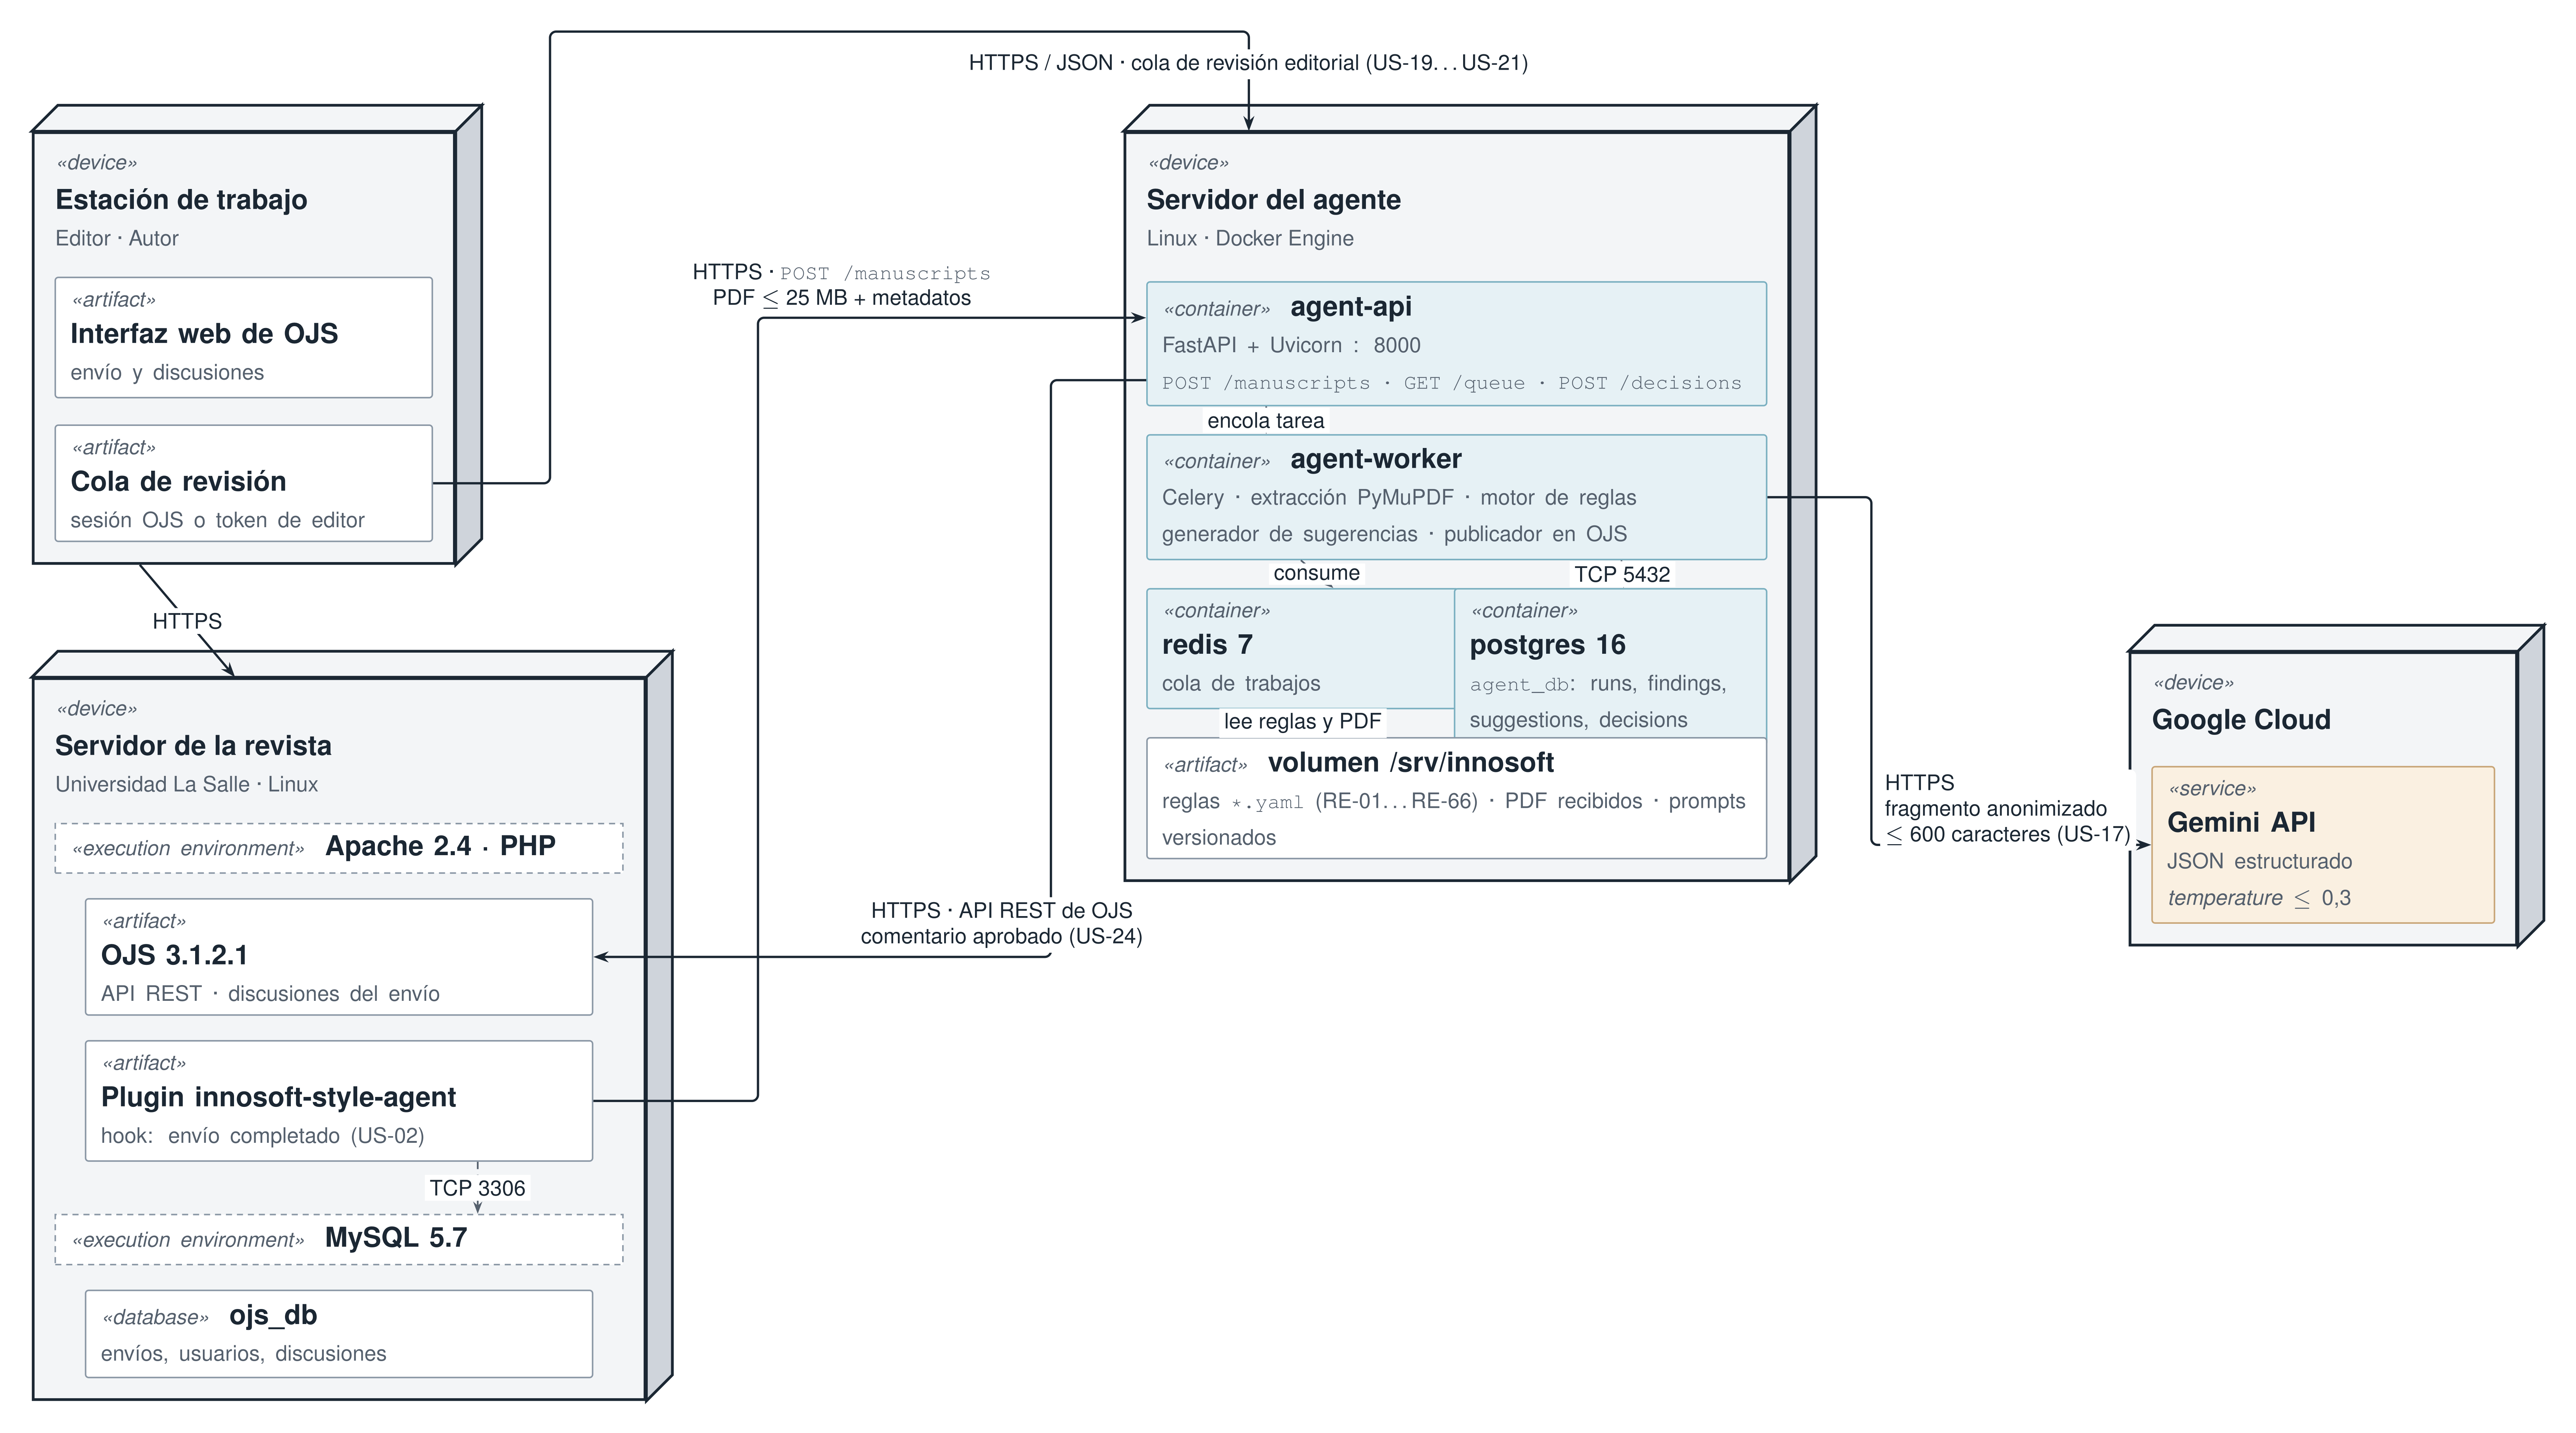
\includegraphics[width=\textwidth]{figuras/despliegue_innosoft.png}
  \caption{Diagrama de despliegue del agente integrado con OJS}
  \label{fig:despliegue}
\end{figure}

\begin{figure}[H]
  \centering
  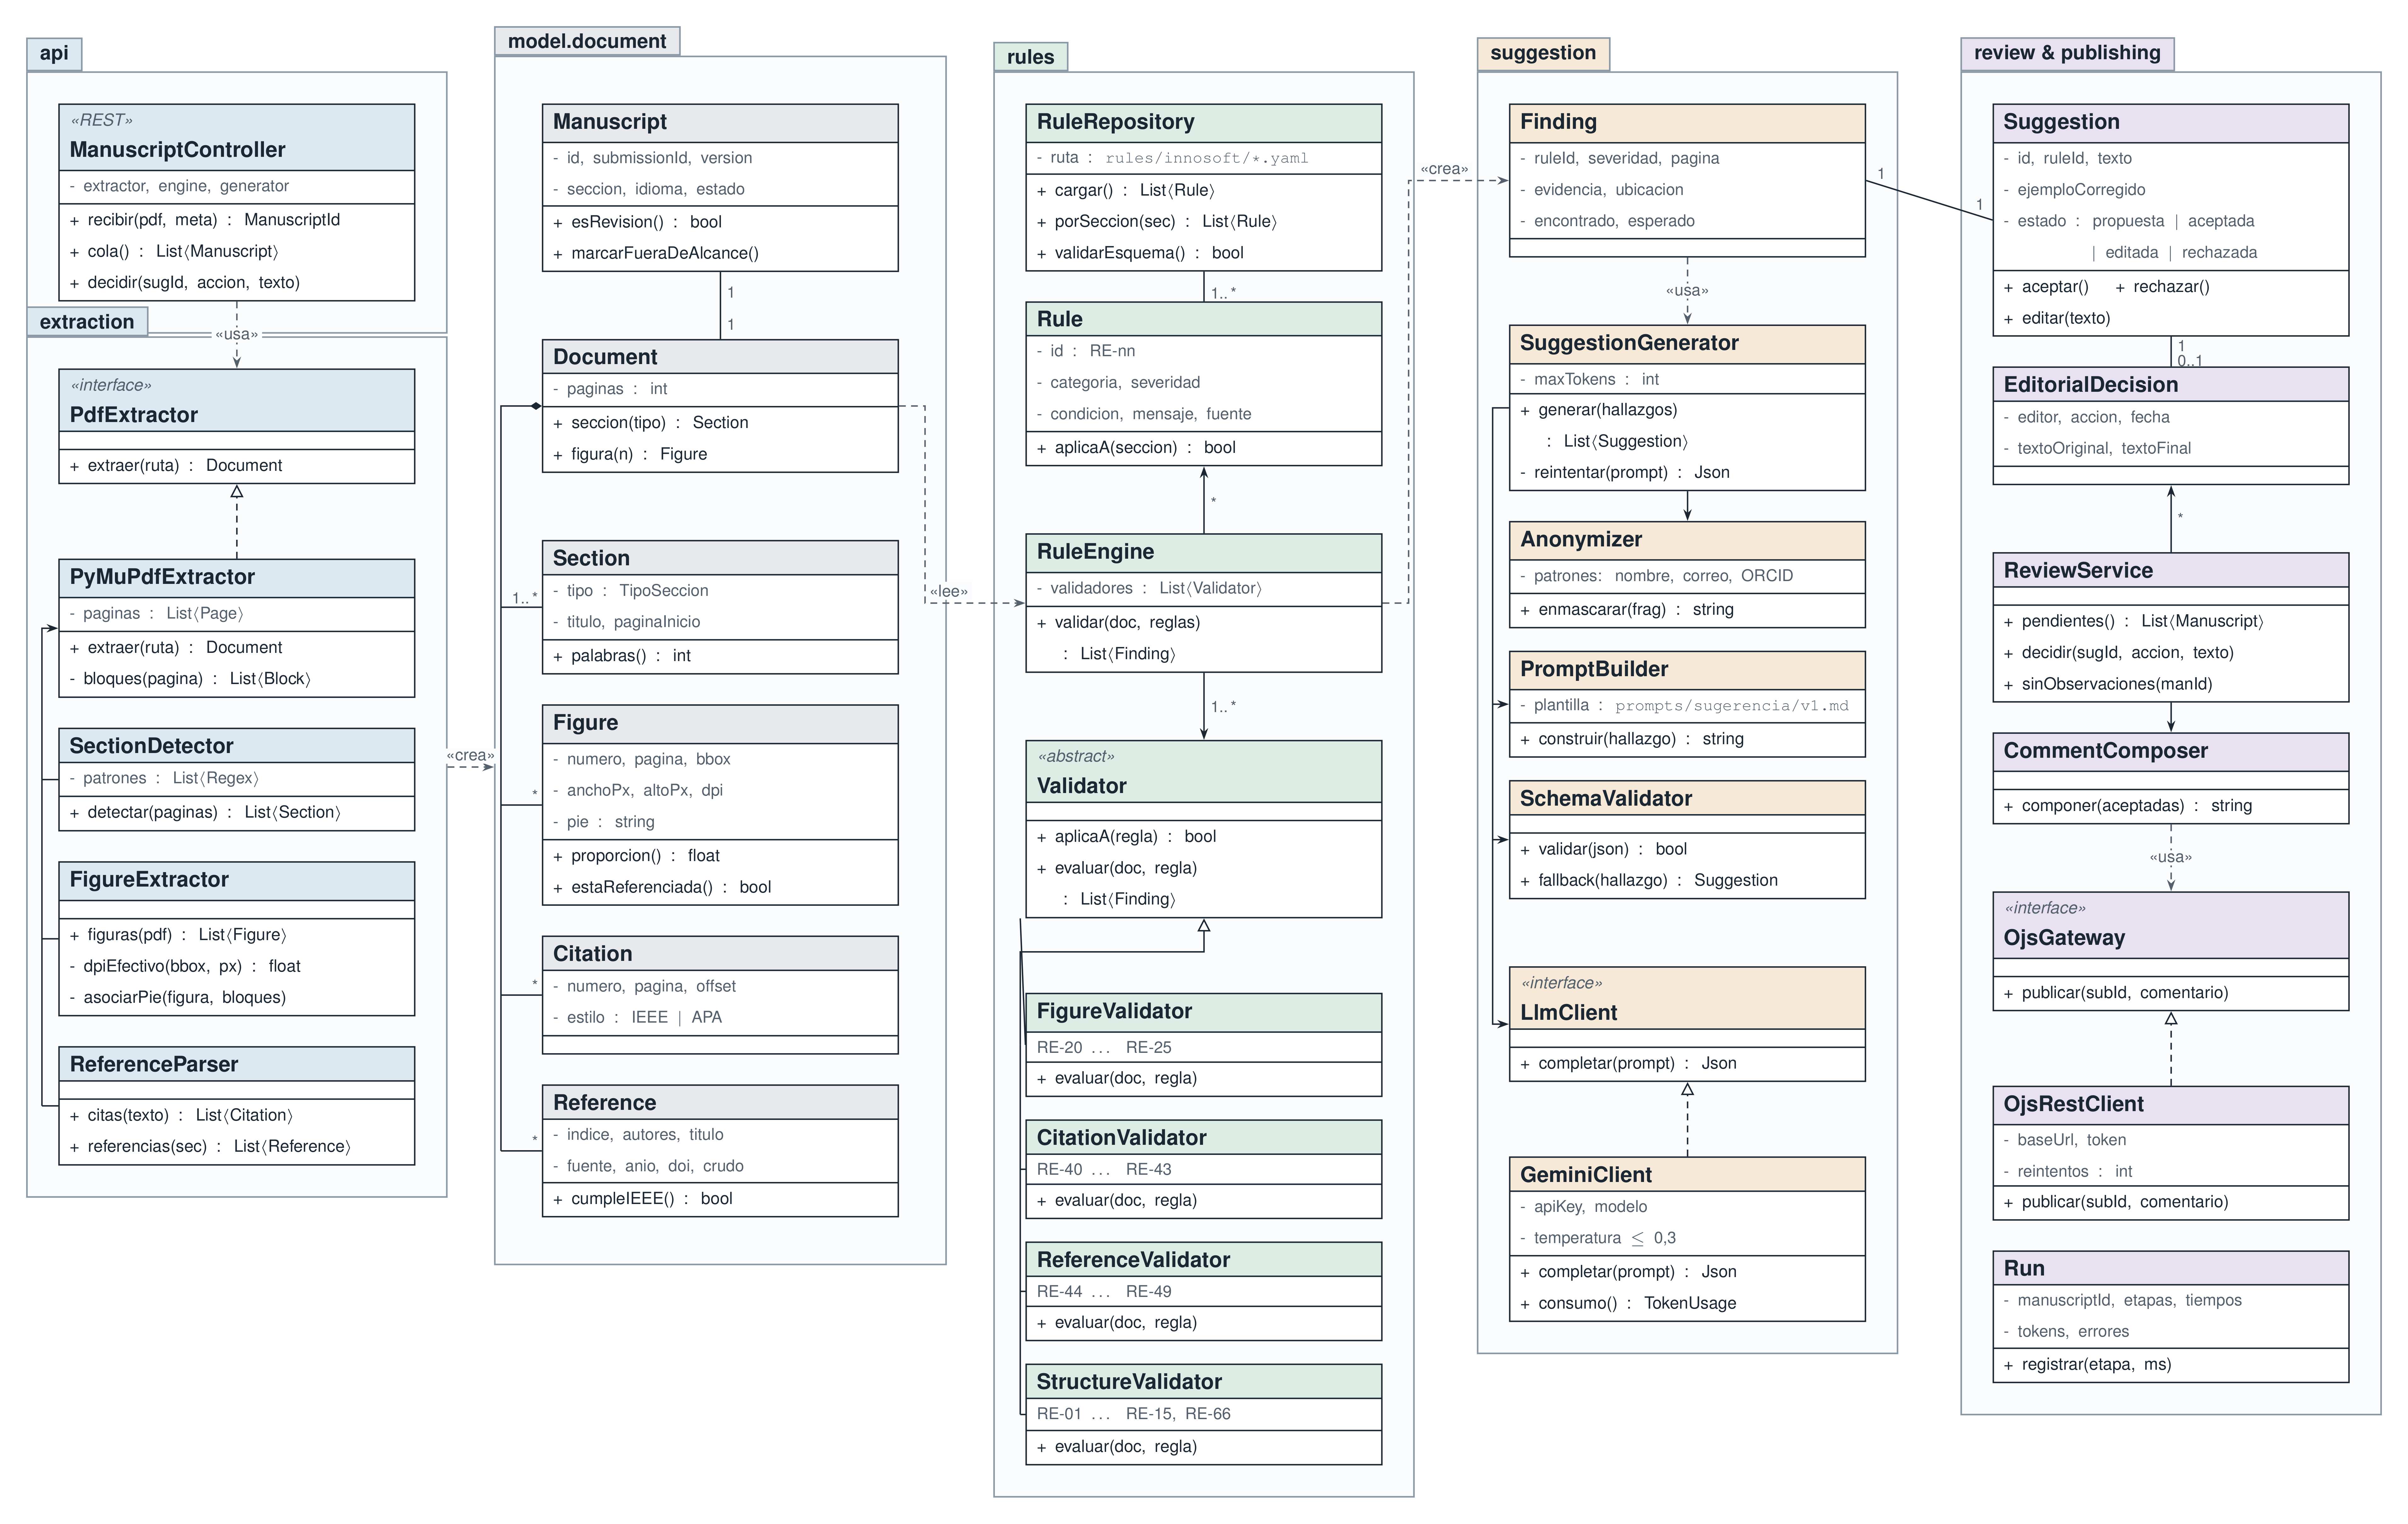
\includegraphics[width=\textwidth]{figuras/clases_innosoft.png}
  \caption{Diagrama de clases del agente}
  \label{fig:clases}
\end{figure}

\section{Plan de iteraciones}

El Sprint 1 que fue del 14 al 25 de septiembre se usó por completo en escribir las especificaciones y hacer el diseño y no produjo código. Por eso el 29 de septiembre se volvió a planificar lo que quedaba del proyecto en cinco sprints que se muestran en la Tabla~\ref{tab:3-2} y en la Figura~\ref{fig:gantt}.

{\small
\begin{longtable}{@{}>{\raggedright\arraybackslash}p{0.114\textwidth}>{\raggedright\arraybackslash}p{0.172\textwidth}>{\raggedright\arraybackslash}p{0.297\textwidth}>{\raggedright\arraybackslash}p{0.311\textwidth}@{}}
\caption{Plan por sprint (fuente: \texttt{priorizacion\_\allowbreak{}rice\_\allowbreak{}sprint1.\allowbreak{}xlsx}, hoja \emph{Replan 29-sep})}\label{tab:3-2}\\
\toprule
\textbf{Sprint} & \textbf{Fechas} & \textbf{Historias} & \textbf{Meta} \\
\midrule
\endfirsthead
\toprule
\textbf{Sprint} & \textbf{Fechas} & \textbf{Historias} & \textbf{Meta} \\
\midrule
\endhead
\bottomrule
\endfoot
\endlastfoot
1 & 14-sep $\rightarrow$ 25-sep & Catálogo, RICE, diagramas, 00-producto, formato-reglas y specs de las 37 historias & Especificación y diseño \\
2 & 29-sep $\rightarrow$ 09-oct & US-00, US-01, US-04, US-09, US-06, US-10 & \emph{Walking skeleton} en Docker con RE-20/RE-21 \\
3 & 12-oct $\rightarrow$ 23-oct & US-03, US-05\textbackslash\{\}\emph{, US-07, US-08\textbackslash\{\}}, US-11\textbackslash\{\}\emph{, US-12, US-13\textbackslash\{\}} + \emph{spike} OJS & Citas y referencias IEEE detectadas; decisión técnica sobre OJS \\
4 & 26-oct $\rightarrow$ 06-nov & US-17, US-15, US-16, US-18\textbackslash\{\}*, US-28, US-19, US-20 & Sugerencias con Gemini anonimizadas y visibles para el editor \\
5 & 09-nov $\rightarrow$ 20-nov & US-21, US-24, US-02 & El flujo completo funciona desde OJS hasta el comentario que ve el autor \\
6 & 23-nov $\rightarrow$ 04-dic & Sin historias nuevas & Evaluación (precisión, recall, F1, aceptación), manuales y tesis \\
\end{longtable}
}

Las historias marcadas con asterisco entran al producto mínimo con un alcance menor al de su especificación completa.

\begin{itemize}
  \item US-05 solo detecta Resumen Palabras clave y Referencias.
  \item US-08 separa las referencias en entradas pero no las parte en campos.
  \item US-11 solo cubre las reglas RE-23 y RE-24.
  \item US-13 solo cubre las reglas RE-44 RE-46 RE-47 y RE-49.
  \item US-18 hace reintentos pero no controla el presupuesto de tokens.
\end{itemize}

Si el proyecto vuelve a atrasarse se recorta en este orden. Primero sale el plugin de OJS de US-02 y el análisis se dispara a mano. Después US-11 pasa completa a la entrega R2. Después US-13 queda solo con RE-44 y RE-46. Y por último la evidencia que muestra US-20 queda solo en texto sin miniaturas.

\begin{figure}[H]
  \centering
  \begin{ganttchart}[
      x unit=1.2mm, y unit chart=0.65cm, y unit title=0.55cm,
      hgrid, vgrid={*{6}{draw=none}, dotted}, canvas/.style={draw=gray!50},
      time slot format=isodate,
      title/.style={fill=gray!15, draw=gray!50},
      title label font=\scriptsize,
      bar/.style={fill=gray!60, draw=gray!80},
      bar label font=\footnotesize,
      bar height=0.55,
      milestone/.style={fill=black, draw=black},
      milestone label font=\footnotesize]{2026-09-14}{2026-12-04}
    \gantttitle{Sep}{17}\gantttitle{Oct}{31}\gantttitle{Nov}{30}\gantttitle{Dic}{4} \\
    \ganttbar{S1 Especificación y diseño}{2026-09-14}{2026-09-25} \\
    \ganttbar{S2 Walking skeleton}{2026-09-29}{2026-10-09} \\
    \ganttbar{S3 Citas, referencias y spike OJS}{2026-10-12}{2026-10-23} \\
    \ganttbar{S4 Gemini e interfaz editorial}{2026-10-26}{2026-11-06} \\
    \ganttbar{S5 Revisión y publicación en OJS}{2026-11-09}{2026-11-20} \\
    \ganttbar{S6 Evaluación, manuales y tesis}{2026-11-23}{2026-12-04} \\
    \ganttmilestone{Hitos: demo (09-oct), flujo en OJS (20-nov)}{2026-10-09}
    \ganttmilestone{}{2026-11-20}
  \end{ganttchart}
  \caption{Diagrama de Gantt de los sprints según la planificación del 29 de septiembre de 2026}
  \label{fig:gantt}
\end{figure}

\section{Recursos requeridos}

{\small
\begin{longtable}{@{}>{\raggedright\arraybackslash}p{0.125\textwidth}>{\raggedright\arraybackslash}p{0.287\textwidth}>{\raggedright\arraybackslash}p{0.241\textwidth}>{\raggedright\arraybackslash}p{0.241\textwidth}@{}}
\toprule
\textbf{Tipo} & \textbf{Recursos} & \textbf{Uso} & \textbf{Disponibilidad} \\
\midrule
\endfirsthead
\toprule
\textbf{Tipo} & \textbf{Recursos} & \textbf{Uso} & \textbf{Disponibilidad} \\
\midrule
\endhead
\bottomrule
\endfoot
\endlastfoot
Humanos & Equipo de tesis, asesor, editores de Innosoft, autores participantes & Escribir y revisar reglas, programar el agente, revisar los reportes & Se coordina con la universidad y la participación es voluntaria \\
Tecnológicos & Computadoras personales, instancia de OJS, servidor del agente, PostgreSQL & Programar, integrar con OJS, hacer pruebas y guardar datos & Equipos propios y servicios gratuitos o de bajo costo \\
Software & Python, FastAPI, PyMuPDF, PostgreSQL, Pytest, Docker, Git/GitHub, API de Gemini & Procesamiento, validación, sugerencias, pruebas & Código abierto o tier gratuito \\
Información y datos & Plantillas DOCX/LaTeX, directrices, manuscritos anonimizados, corpus sintético de PDFs & Configurar reglas, probar y medir & Requiere autorización y anonimización (Ley N.º 29733) \\
Económicos & S/ 760 (Tabla~\ref{tab:2-5}) & Cuotas, despliegue, capacitación, impresiones & Financiado por el equipo \\
Metodológicos & Excel RICE, specs SDD, Sprint Backlog, encuestas de validación & Priorizar, especificar, controlar avances, evaluar & Adecuado para un equipo de dos personas \\
\end{longtable}
}

\section{Avance de la implementación}

El avance se registra por historia al cierre de cada sprint, con el estado de su especificación, sus pruebas automatizadas y su commit en el repositorio. Al cierre del Sprint 2 (9 de octubre de 2026) quedó implementado el \emph{walking skeleton} de extracción y validación: recepción de PDF por API con idempotencia (US-01), extracción de texto (US-04) y de figuras con DPI efectivo (US-06), carga de reglas YAML (US-09) y validación de figuras RE-20 y RE-21 con consulta de hallazgos (US-10), sobre el entorno Docker con integración continua (US-00): 6 de 37 historias, 2 de 44 reglas y 4 de 13 endpoints canónicos, con 84 casos de prueba en verde.

\pendiente{al cierre del Sprint 6, actualizar las cifras finales y describir lo construido en los sprints 3 a 6.}

\section{Validación y evaluación}

{\small
\begin{longtable}{@{}>{\raggedright\arraybackslash}p{0.158\textwidth}>{\raggedright\arraybackslash}p{0.231\textwidth}>{\raggedright\arraybackslash}p{0.248\textwidth}>{\raggedright\arraybackslash}p{0.257\textwidth}@{}}
\caption{Criterios de evaluación por objetivo específico}\label{tab:3-3}\\
\toprule
\textbf{Objetivo} & \textbf{Criterio} & \textbf{Método} & \textbf{Meta inicial} \\
\midrule
\endfirsthead
\toprule
\textbf{Objetivo} & \textbf{Criterio} & \textbf{Método} & \textbf{Meta inicial} \\
\midrule
\endhead
\bottomrule
\endfoot
\endlastfoot
OE1 -- Arquitectura & Módulos integrados y reglas aplicadas por revista & Prueba del flujo completo: recepción $\rightarrow$ reporte $\rightarrow$ comentario en OJS & Flujo de punta a punta en el Sprint 5 \\
OE2 -- Análisis documental & Reconocimiento de secciones, figuras, citas y referencias & Comparación con anotación manual sobre un corpus & Recall por regla $\geq$ 0,75 en reglas D \\
OE3 -- Validación y reporte & Precisión y utilidad de las sugerencias & Precisión por regla; aceptación / edición / rechazo por los editores & Precisión $\geq$ 0,85 en reglas D; aceptación $\geq$ 70 \% \\
OE4 -- Evaluación & Tiempo de análisis y de revisión estilística & Medición en \texttt{runs} (US-28) y comparación manual vs. asistida & Análisis < 3 min para 15 páginas (RNF-03); \pendiente{definir instrumento y meta de reducción del tiempo de revisión — el borrador proponía 20 \%} \\
Usabilidad del reporte & Claridad y aplicabilidad para autores y editores & Encuesta breve o juicio de expertos & Reporte valorado como útil \\
\end{longtable}
}

Las metas son propuestas del equipo y se confirman con el asesor antes del Sprint 6 (\texttt{specs/\allowbreak{}00-producto.\allowbreak{}md} §1). \pendiente{corpus anotado — número de manuscritos históricos y autorización (00-producto §18).}

\section{Aspectos éticos y protección de datos}

Los manuscritos reales pueden contener datos personales de los autores (nombres, correos, ORCID, afiliaciones). Por la Ley N.º 29733, (i) se guardan fuera del repositorio (\texttt{muestras/\allowbreak{}} en \texttt{.\allowbreak{}gitignore}), (ii) las pruebas automatizadas usan PDFs sintéticos generados con PyMuPDF, y (iii) a Gemini solo sale un fragmento de hasta 600 caracteres anonimizado, con registro de lo enviado (US-17, RNF-02).
